\documentclass[border=3pt]{standalone}
\usepackage{tikz}
\usetikzlibrary{arrows.meta,calc}
\tikzset{pin/.style={-{Stealth[length=5pt]}},
  blk/.style={draw, thick, minimum width=26mm, minimum height=26mm, font=\sffamily\small, align=center}}
\begin{document}
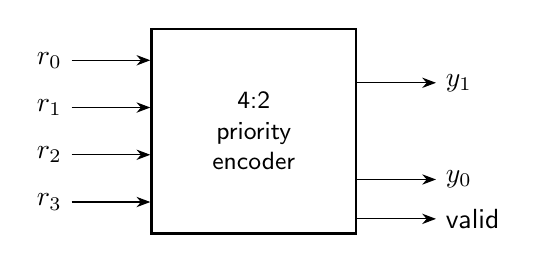
\begin{tikzpicture}[font=\sffamily]
  \node[blk] (e) {4:2\\priority\\encoder};
  \foreach \i/\dy in {0/9mm,1/3mm,2/-3mm,3/-9mm}{
    \draw[pin] ($(e.west)+(-10mm,\dy)$) node[left]{$r_\i$} -- ($(e.west)+(0,\dy)$);}
  \draw[pin] ($(e.north east)+(0,-7mm)$) -- ++(10mm,0) node[right]{$y_1$};
  \draw[pin] ($(e.south east)+(0,7mm)$) -- ++(10mm,0) node[right]{$y_0$};
  \draw[pin] ($(e.south east)+(0,2mm)$) -- ++(10mm,0) node[right]{valid};
\end{tikzpicture}
\end{document}
